\documentclass[12pt]{article}

\usepackage{graphicx}
\usepackage{bytefield}
\usepackage{makecell}
\usepackage{tcolorbox}
\usepackage{etoolbox}
\usepackage[]{hyperref}
%\usepackage[]{authblk} 


%\renewcommand\Authfont{\fontsize{12}{14.4}}
%\renewcommand\Authfont{\small}


\title{The Gateway Protocol\\ \small v0.1.1}


\author{
        \small Martin Riedel\\
        \small \texttt{martin@identity.org}
        \and
        \small Seamus Hennessy\\
        \small \texttt{seamus.hennessy@identity.org}
        \and
        \small Phillip Shoemaker\\
        \small \texttt{phillip@identity.org}
}
\date{\today}


%\usepackage{draftwatermark}
%\SetWatermarkText{Confidential\\ \small \date{\today}}
%\SetWatermarkScale{5}
%\SetWatermarkColor[gray]{0.95}


\hypersetup{
    pdftitle={The Gateway Protocol},
    pdfauthor={martin@identity.org},
    pdfsubject={blockchain},
    pdfkeywords={blockchain, protocol, dao},
    bookmarksnumbered=true,
    bookmarksopen=true,
    bookmarksopenlevel=1,
    colorlinks=true,
    pdfstartview=Fit,
    pdfpagemode=UseOutlines,    % this is the option you were lookin for
    pdfpagelayout=TwoPageRight
}

\definecolor{light-gray}{gray}{0.85}


\begin{document}

\maketitle

\begin{abstract}
The \textit{Gateway Protocol} is a decentralized, semi-trustless protocol that governs the lifecycle of Gateway Passes (GP), Gatekeeper Networks (GKN) and associated participants like Gatekeepers (GP issuers), users (GP Holders) and integrating dApps (GP verifiers). A gateway pass is a pseudonymous property that is uniquely bound to a gatekeeper network and represents the adherence of a user (represented by a wallet or identifier) to a predetermined set of requirements (framework). Decentralized applications (dApps) are able to integrate into an existing gatekeeper network in a permissionless way and protect their interface by only allowing the interaction of users with existing and valid gateway passes. Gatekeepers are the issuers of gateway passes within a specific GKN and are responsible for the proper verification of users and the issuance of GPs. The Gateway Protocol further supports the value flows around GP lifecycle events that allow Gatekeepers to be reimbursed for their service and the network to collect an operating fee. The Gateway Protocol implements a governance token (CVC) that secures the ecosystem through staking mechanisms. Lastly, a DAO of governance token holders will allow the community to participate in future iterations of the protocol. The Gateway Protocol is a cross-chain protocol, with governance processes of the protocol being restricted to a single ledger.
\end{abstract}

\normalsize

% Introduction
\section{Protecting DeFi Values in a (Soon to be) Regulated World}\label{sec:introduction}

DeFi is growing at an unprecedented rate.\\

At the start of 2020, the ecosystem’s Total Locked Value (TVL) sat at \$630 million. Within 12 months, that figure rose to \$18 billion. By the start of 2022, DeFi’s TVL had hit \$240 billion. That’s a Compound Annual Growth Rate (CAGR) of 1,851\% over two years.\\\\

\begin{figure}[h]
  \begin{center}
    \centering
    \includegraphics[width=100mm,scale=0.5]{figures/01-introduction-defi-lama.png}
    \caption[Fig 1]{\href{https://defillama.com/}{DeFi Llama}, DeFi industry analyst.\label{fig:defi-tvl}}
  \end{center}
\end{figure}

This meteoric rise reflects the speed with which individuals, traders, companies, and other groups have identified the opportunities and advantages created by DeFi. For example:
\begin{itemize}
\item Protecting individuals’ privacy while accessing financial services.
\item Eliminating unnecessary intermediaries.
\item Cutting out human foul play with smart contracts.
\item Trustless and decentralized architecture.
\end{itemize}

However, for all the good it brings, DeFi has also caught the attention of two other groups:
\begin{enumerate}
\item Bad actors, e.g., organized crime and terrorist groups, and insider traders
\item Regulators
\end{enumerate}
The same characteristics that make DeFi attractive to legitimate individuals and organizations also attract the worst aspects of humanity—and the organizations set up to protect against them.

\subsection{DeFi Attracts Unwanted Attention Due to Lack of KYC and AML}

The simple fact is that criminals and other bad actors thrive in economic environments that lack adequate controls to identify and exclude them. This is why organizations like the Financial Action Task Force (FATF) exist—to advise regulators on the policies needed to (as far as possible) cut bad actors out of their financial systems.

FATF—an intergovernmental group founded on the initiative of the G7 summit in 1989—produced the original recommendations for Anti-Money Laundering (AML) regulations in 1990. The regulations that sprang from these recommendations were bolstered by the 2001 Patriot Act following the 9/11 terrorist attacks, which coined the term KYC: Know Your Customer. FATF has updated its recommendations several times in the intervening years. Today, most countries employ some version of the group’s recommended AML and KYC regulations.

However, so far, DeFi has been minimally affected by regulation. While some individual DeFi protocols operate basic KYC checks, they typically aren’t well implemented and don’t significantly impede bad actors. Worse, due to poor implementation, they often place users’ personal data at risk and run contrary to the privacy principles of DeFi.

Given the explosion of interest—and capital—in DeFi protocols, the ecosystem has inevitably attracted the attention of bad actors and regulators.

\subsection{What Problems Does a Lack of KYC/AML Cause?}
Beyond attracting unwanted attention, DeFi’s lack of KYC and AML creates three huge problems:

\begin{enumerate}
\item \textbf{It keeps big players out of the ecosystem}\\
Currently, many regulated market makers are effectively shut out of the DeFi ecosystem. While DeFi doesn’t yet have strong regulations, these organizations \emph{do}—and that means they can’t engage in any trades without knowing who their counterparties are.

\item \textbf{It limits liquidity}\\
The exclusion of major market makers means less liquidity in the ecosystem and therefore fewer money-making opportunities for everybody.

\item \textbf{It harms trust in DeFi trading}\\
It isn’t possible to interact through a DeFi marketplace with the assurance that counterparties aren’t bad actors. Since most individuals and organizations would prefer not to trade with criminals or terrorists, this uncertainty undoubtedly impacts DeFi’s reputation—and possibly its uptake.

\end{enumerate}

\subsection{Regulations are Imminent}
There is no doubt that KYC and AML regulations for DeFi are imminent. Some self-proclaimed DeFi providers may already fall under FATF’s revised definition of a Virtual Asset Service Provider (VASP). FATF guidance from October 2021 notes that:

\begin{figure}[htbp]
\begin{quote}
\centering
"[...] creators, owners and operators or some other persons who maintain control or sufficient influence in the DeFi arrangements [...] may fall under the FATF definition of a VASP where they are providing or actively facilitating VASP services."
\caption{FATF, \href{https://www.fatf-gafi.org/publications/fatfrecommendations/documents/guidance-rba-virtual-assets-2021.html}{Updated Guidance} for a Risk-Based Approach to Virtual Assets and Virtual Asset Service Providers~\cite{fatf-guidance}.\label{cap:fatf-guidance}}
\end{quote}
\end{figure}

This would make them subject to the infamous \emph{Travel Rule}, which requires the collection of identifying information on the originators and beneficiaries of domestic and cross-border wire transfers—including names, account numbers, and physical addresses.

Again, while FATF guidance isn’t immediately binding, regulators worldwide take it seriously—and it is usually enshrined in law by most developed nations in close to unchanged form.

The facts are simple: DeFi regulation is coming—initially as KYC/AML requirements, but ultimately in the form of regulations designed to protect investors (e.g., from insider trading) and block bad actors in a similar manner to that used in traditional financial markets.

\subsection{Protecting Core DeFi Values}
Given that regulation is inevitable, the aim should be to identify a solution that satisfies dApps’ new regulatory requirements \emph{without} hindering basic DeFi values of privacy and decentralization.

\begin{tcolorbox}[width=\textwidth,colback={light-gray},title={\textbf{Privacy vs. Anonymity (and Why it Matters)}},colbacktitle=light-gray,coltitle=black]
It’s a popular misconception that DeFi allows individuals to trade anonymously. Blockchain as a whole at best offers pseudo-anonymity. Since wallet IDs remain constant, users must constantly protect against their identities being linked to a wallet address—something that would typically be trivial for a government agency.

In practice, well-designed dApps provide individuals with privacy. It is typically possible to trade between counterparties without either side knowing the identity of the other. This privacy component of DeFi must be protected when seeking solutions to upcoming regulations.
\end{tcolorbox}

This white paper proposes the Gateway Protocol as a solution to allow dApps to meet upcoming KYC and AML requirements without:

\begin{enumerate}
\item Developing user verification capabilities internally.
\item Viewing or holding any personal information on users.
\item Directly interacting with regulators in most cases.
\end{enumerate}

In doing so, the Gateway Protocol will protect DeFi users’ privacy while enabling the positive impact of upcoming regulations. Similarly, the Gateway Protocol operates as a DAO and is governed via a voting system that anyone can join, ensuring the solution remains as decentralized as possible.

\subsection{Benefits for the DeFi Community}

By addressing the needs of regulators while protecting DeFi values, the Gateway Protocol will benefit all DeFi stakeholders:
\begin{itemize}
\item \textbf{Regulators} can ensure bad actors are (as far as possible) excluded from the DeFi ecosystem.
\item \textbf{dApps} can adhere to new KYC/AML regulations without developing those capabilities internally.
\item \textbf{Regulated institutions} can join the DeFi ecosystem while satisfying existing KYC/AML regulations.
\item \textbf{Legitimate DeFi adopters} can trade freely without worrying that counterparties may be bad actors.
\item \textbf{All DeFi stakeholders} can benefit from increased liquidity and reduced influence of bad actors such as criminal and terrorist groups and insider traders.
\end{itemize}


% Gateway Protocol Solution
\section{Gateway Protocol Solution Overview}\label{sec:solution}
The Gateway Protocol is a cross-chain oracle token model that enables any application operating on a decentralized ledger (i.e., a dApp) to add a permissioning layer that adheres to predetermined requirements. The protocol allows dApps to meet AML/KYC requirements of an industry or location without developing their own systems for identity verification or secure data storage.

Identity verification is completed by one or more Gatekeepers belonging to a Gatekeeper network. Each Gatekeeper network will enforce a specific set of requirements, which may be modeled on a set of trading regulations, e.g., those active in a DEX user’s country of residence. Requirements may include age, country of residence, IP address, investor status, and more. Once a Gatekeeper has verified an individual’s identity and conformance with the requirements, it will issue them with a Gateway Pass.

To take part in the ecosystem, a dApp simply extends its existing interfaces to require the presence of a specific and active Gateway Pass within an individual’s wallet. If the appropriate Pass is present and active, the individual can interact with the dApp as usual. If a Pass isn’t present, the individual is first directed to an appropriate Gatekeeper network to undergo the verification process.

The Gatekeeper Protocol is managed by a Decentralized Autonomous Organization (DAO), which decides on the evolution of the protocol. The DAO is involved in operational decisions like the appointment of Guardians and maintenance of Gatekeeper network processes. The DAO operates via a voting system, allowing Governance Token holders to propose and vote on changes to the Ecosystem.

Gateway Protocol contracts can be deployed on any compatible chain, allowing integration on a wide range of Blockchains and Applications.

\subsection{Personas in the Gateway Pass Ecosystem}

There are three primary personas within the ecosystem: \textbf{dApps}, \textbf{Gatekeepers}, and \textbf{Gateway Pass Users}. These personas will play a direct role in issuing, using, and verifying Gateway Passes.

Two further personas play a supporting role: \textbf{Gateway Pass Holders} and \textbf{Guardians}. These personas will enable the operations and continued maintenance of individual Gatekeeper networks through voting, admitting new gatekeepers, etc.

\subsubsection{dApps (Gateway Pass Verifiers)}
dApps are the primary beneficiaries of the Gateway Protocol. It enables a dApp to adhere to any set of KYC/AML requirements without developing its own verification process. Instead, a dApp verifies the presence and validity of a relevant Gateway Pass before allowing a User to access the service.

\begin{figure}[h]
  \begin{center}
    \centering
    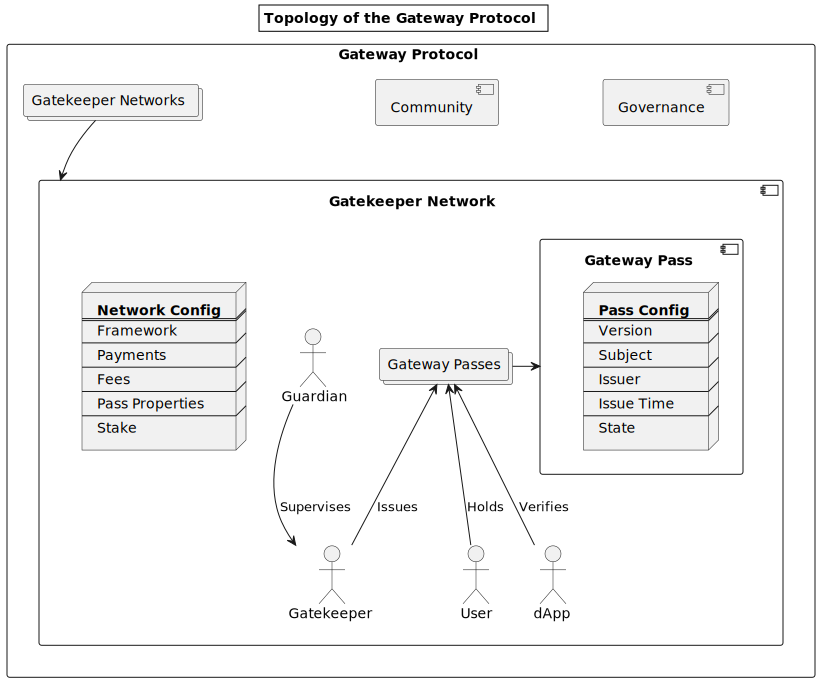
\includegraphics[width=0.8\textwidth]{figures/02-solution-topology.pdf}
    \caption[Fig 3]{Topology and components of the Gateway Protocol}
  \end{center}
\end{figure}

To take part, a dApp integrates with one or more Gatekeeper networks and establishes a Custodial Wallet from which Gatekeepers can draw any funds they are owed for using verified Gateway Passes by that Gatekeeper. This process will be explained in more detail in the ‘Gatekeeper Incentives’ section.

\vspace{1em}

\textbf{Motivation:}
\begin{itemize}
\item Easily adhere to any set of legal, regulartory or technical requirements.
\item Externalize the verification and enforcement of framework rules to the Gatekeeper network
\end{itemize}

\textbf{Role in the Ecosystem:}
\begin{itemize}
\item Funds the verification process through payments to Gatekeepers. This cost can be offset to Users of the dApp.
\item May also participate in Protocol governance by staking as a Governance Token Holder.
\end{itemize}

\subsubsection{Gatekeepers (Gateway Pass Issuers)}
A Gatekeeper is any legal entity that can fulfill the requirements of a Gatekeeper network. Each Gatekeeper's ability to do so is verified and audited by the Guardian on an ongoing basis.

Gatekeepers are the service providers of the Gateway Protocol. Each Gatekeeper belongs to one or more Gatekeeper networks and is responsible for enforcing the requirements of those networks by verifying users per those requirements—for example, by verifying a User’s age and location.

Gatekeepers are also involved in the governance of Gatekeeper networks and have a vested interest in maintaining each network’s requirements in line with any relevant regulations or frameworks.

\vspace{1em}

\textbf{Motivation:}
\begin{itemize}
\item Gatekeepers are compensated for Verification Services or Gateway Pass utilization in governance tokens.
\end{itemize}

\textbf{Role in the Ecosystem:}
\begin{itemize}
\item Completes the User verification process.
\item Issues, Freezes, and Revokes Gateway Pass in accordance with a User’s compliance (or lack of compliance) with a Gatekeeper network’s requirements.
\end{itemize}

\subsubsection{Gateway Pass Users}
Gateway Pass Users are individuals who wish to interact with a dApp that is part of the Gateway Pass ecosystem.

\vspace{1em}

\textbf{Motivation:}
\begin{itemize}
\item Users must acquire a Gateway Pass from a relevant Gatekeeper network before accessing services offered by participating dApps.
\item Evidence provided to a Gatekeeper by the User is protected and remains private and apart from a pseudonymous Gateway Pass, no personal information is put in the public space.
\end{itemize}

\textbf{Role in the Ecosystem:}
\begin{itemize}
\item Must approach a Gatekeeper from a relevant Gatekeeper network and provide requested evidence to satisfy the network’s requirements.
\end{itemize}

\subsubsection{Voters (Governance Token Holders)}
Voters maintain the DAO Ecosystem by proposing and voting on changes. Any individual or organization that holds Gateway Passes has the right to vote on proposals. Staking will be required to propose a change to the DAO Ecosystem.

Gatekeepers will usually also be voters, as they have a vested interest in protecting, updating, and introducing requirements. Guardian Governance may transition to voters to further decentralize the Ecosystem in the future.

\vspace{1em}

\textbf{Motivation:}\\
Any party with an interest in the Gateway Protocol and/or DAO Ecosystem has a vested interest in ensuring its continued operation and effectiveness. Holding Governance Tokens provides parties with the opportunity to influence these operations.

\vspace{1em}

\textbf{Role in the Ecosystem:}\\
Proposing and voting on changes, such as:
\begin{itemize}
\item Proposing a new Gatekeeper network with predefined requirements.
\item Changing the requirements of an existing Gatekeeper network.
\item Supporting Governance Token utilization.
\end{itemize}

\subsubsection{Guardian}
The Guardian supervises the ecosystem and protocol and ensures each Gatekeeper network correctly adheres to its requirements.

\vspace{1em}

\textbf{Motivation:}
\begin{itemize}
\item Are experts in a specific regulatory or legal framework and want to enable compliance in a web3-context.
\item Fee-based income model through network operations and Gatekeeper staking.
\end{itemize}

\textbf{Role in the Ecosystem:}
\begin{itemize}
\item Regularly audits Gatekeepers on their off-chain verification and evidence data.
\item Slashes Governance Token stake for Gatekeepers that fail to meet requirements.
\item Removes Gatekeepers that continually fail to meet requirements or act maliciously.
\item Audits and accepts new Gatekeepers into Gatekeeper networks.
% \item Maintains on-chain smart contracts for the Gateway Protocol.
\item Supports Governance Token utilization.
\end{itemize}

\subsection{What is a Gatekeeper Network Framework?}
A Gatekeeper network framework is the set of requirements a User must meet to obtain a Gateway Pass from a Gatekeeper. Similarly, the framework is also the set of requirements a Gatekeeper must enforce before issuing a Gateway Pass.

Each framework will have its own Gatekeeper network, and each Gatekeeper network will only enforce one framework. However, a Gatekeeper can be part of as many Gatekeeper networks as desired, so long as it is competent to enforce the associated framework and prove that to the Guardian.

\subsection{End User Experience}
Users that already have a relevant Gateway Pass in their wallet can interact seamlessly with participating dApps with no additional steps. Users that don’t already have a relevant Pass will be directed to the appropriate Gatekeeper network—ideally providing them with several Gatekeepers to choose from—where they will undergo the verifications needed to issue a Pass.

The verification process will vary depending on the framework of the relevant Gatekeeper network. For example, some dApps may require users to undergo a stringent identity verification process, while others may simply need proof that the User is over a certain age.\\


% Tokens of the Gateway Protocol
\section{Passes and Tokens of the Gateway Protocol}\label{sec:tokens}
The Gateway Protocol requires the use of two distinct token types: the Gateway Pass, and the Governance Token.

\subsection{The Gateway Pass}
The Gateway Pass (GT) lies at the heart of the Gateway Protocol. Each Gatekeeper network will issue its own unique type
of Gateway Pass to verified users. The presence of a Gateway Pass in a User’s wallet is proof that an off-chain
verification has been performed by a Gatekeeper in line with the requirements of its network’s framework.

This process allows dApps to interact with verified users without needing to conduct the verification or hold any
personal information. Instead, dApps simply check each User’s wallet for a Gateway Pass from an appropriate Gatekeeper
network. Participating dApps will require the presence of an active Gateway Pass—and block Users without an active Pass
in their wallet.

dApps do not need to know when a Gateway Pass was issued or which Gatekeeper issued it. So long as the Pass is present
and active, that is proof the User has been verified in line with the appropriate framework requirements. This mechanism
allows dApps to remain accessible and maintain the DeFi ethos while also introducing a needed permissioning layer.

dApps are not limited to accepting Gateway Passes from a single Gatekeeper network. If there are several networks
enforcing requirements that meet a dApp’s permissioning needs, it can choose to simultaneously support all of their
Gateway Passes.

The Gateway Pass States are shown in Table \ref{tbl:gt-states}.
\clearpage

\begin{table}[h]
\begin{tabular}{|m{0.15\textwidth}|m{0.85\textwidth}|}
\hline
\textbf{Active} & Gateway Passes remain active for a period determined by the network framework. After that period, Passes become expired.\\
\hline
\textbf{Expired} & All Passes will expire after a period determined by the issuing Gatekeeper network, which is equal to or less than the absolute limit defined by the Gateway Protocol. To reset expiration, a User must fulfill the same requirements as during the initial Token issuance.\\
\hline
\textbf{Frozen} & Where a Gatekeeper needs to investigate Gateway Pass activity, Passes can be temporarily Frozen. This prevents new activity with participating dApp until the Token is Unfrozen. E.g., A User travels to a different country and has a new IP address, so the Token is frozen while a Gatekeeper reverifies the User.\\
\hline
\textbf{Revoked} & Passes that are misused by bad actors are revoked and become unusable.\\
\hline
\end{tabular}
\caption{\label{tbl:gt-states}Gateway Pass States of the Gateway Protocol.}
\end{table}

\begin{figure}[h]
  \begin{center}
    \centering
    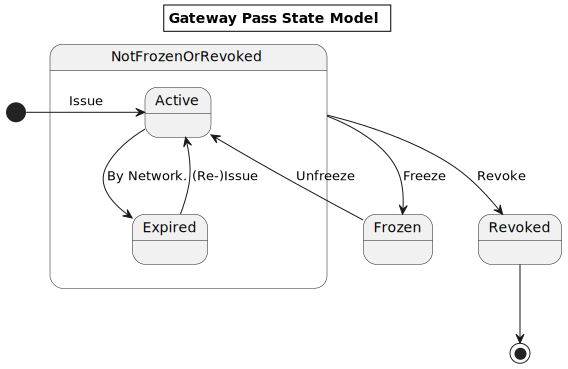
\includegraphics[width=100mm,scale=0.5]{figures/03-pass-state-diagram.pdf}
    \caption[Fig 2]{State Transitions of a Gateway Pass.}
  \end{center}
\end{figure}

\subsection{The Governance Token}
The Gateway Protocol’s native Governance Token is CVC. All Governance Tokens are held and staked on the Solana chain as this is where all governance activities take place.

The Governance Token will be used by two groups:
\begin{enumerate}
\item Ownership of Governance Tokens is a requirement for any individual to become and remain a \textbf{Voter} within the Gateway Protocol. Ownership allows any individual permissionless participation in the Gateway Protocol’s decision processes.
\item Staking Governance Tokens is a requirement for an organization to become and remain a \textbf{Gatekeeper} within any Gatekeeper network. The staking requirement incentivizes Gatekeepers to avoid acting maliciously.
\end{enumerate}

The Governance Token also enables the establishment of a fee structure to fund future protocol development. The Governance Token will not be used to reward any group within the Gateway Protocol—it is purely intended to support governance processes.



% The Gatekeeper Role
\section{The Gatekeeper Role}\label{sec:gatekeeper}
Gatekeepers are critical to the Gateway Protocol’s operation. They provide the compliance, KYC, or identity verification service that dApps need to ensure they comply with any appropriate rules or regulations in their sector or geographic area.

Each Gatekeeper belongs to one or more Gatekeeper networks and completes User verification in line with these networks’ Governance frameworks. It is this verification that enables dApps to transact with users while fulfilling two needs:

\begin{enumerate}
\item Ensuring the User is legally eligible to enter into the transaction; and,
\item Maintaining the User’s privacy.
\end{enumerate}

\begin{figure}[h]
  \begin{center}
    \centering
    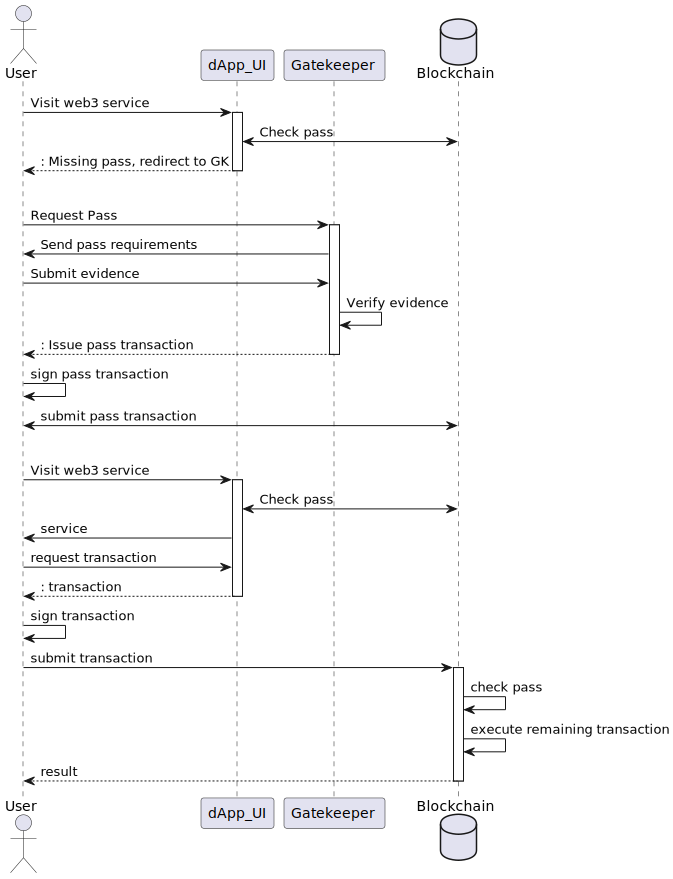
\includegraphics[width=100mm,scale=0.5]{figures/04-sequence-diagram.pdf}
    \caption{Sequence diagram for obtaining a Gateway pass from a Gatekeeper and verifying it within a dApp application}
  \end{center}
\end{figure}

Simply, Gatekeepers removes the burden of KYC/compliance verification from the dApp, so it can transact with users with confidence without reviewing or holding any personal data.

Gatekeepers are also key players in the governance of Gatekeeper networks.

\subsection{What is a Gatekeeper?}
A gatekeeper is a legal entity that enables the Gateway Protocol by completing compliance/KYC checks on users. When a Gatekeeper successfully verifies a User’s compliance with an appropriate Gatekeeper network’s framework, it issues the User with a Gateway Pass.

Gatekeepers operate as oracles that bridge the trust layer between off-chain credential trust—and possibly other verification requirements not directly related to credentials—and the on-chain dApps that require the trusted information to be part of a permissioned Pass.

Most Gatekeepers will likely be organizations that already have KYC and identity verification capabilities for use in traditional financial transactions. The Guardian will regularly audit Gatekeepers to ensure these capabilities are robust and repeatable and remain so over time.
The Guardian will also ensure Gatekeepers adhere to the requirements set by any networks they participate in, which may change over time.

\subsection{Becoming a Gatekeeper}

To become a Gatekeeper within a Gatekeeper network, an organization must go through four steps:

\begin{enumerate}
\item Ensure it has the necessary capabilities to complete appropriate User verifications for a specific Gatekeeper network.
\item Apply to join the Gatekeeper network.
\item Undergo an audit by the Guardian to ensure the necessary capabilities are in place. Audits may also be completed by an authorized third party authorized by the Guardian, e.g., an external accounting firm.
\item Stake a specified minimum amount of Governance Tokens, determined by the volume of Gateway Pass operations they will perform.
\end{enumerate}

Once these four steps are completed, the organization joins the desired Gateway network(s) and can begin offering its verification services to users.

\subsection{Staking}

Staking Governance Tokens will be a requirement for becoming and remaining a Gatekeeper. The stake will incentivize Gatekeepers to uphold their duties and act in the best interest of the Gateway Protocol. There will also be regular Gateway Protocol network fee for Gatekeepers to pay towards the network, which will automatically be taken from existing Gatekeeper stakes.
These fees are used to fund further protocol development and pay Guardians for their supervisory services.

Each Gatekeeper’s Stake exists to ensure the Gatekeeper’s:

\begin{itemize}
\item Service delivery uptime.
\item Proper operation, i.e., only issuing Gateway Passes in line with the relevant Gatekeeper network’s Governance framework.
\item Adherence to Gatekeeper network rules, i.e., maintaining the capabilities needed to be a Gatekeeper within a network.
\item Thorough documentation of operations within the Protocol.
\end{itemize}

The Guardian will have the power to slash the stake of any Gatekeeper that fails to uphold its duties. Examples of infringements that could result in stake slashing include:

\begin{itemize}
\item Falling below a minimum established service delivery uptime.
\item Issuing Gateway Passes to users who do not meet the requirements of a network.
\item Not keeping appropriate records and documentation.
\item Failing audits and/or not remedying audit failures promptly.
\end{itemize}

If a Gatekeeper repeatedly fails to uphold its duties or commits a serious infraction, the Guardian has the power to remove it from the Protocol and slash its outstanding stake.

Gatekeeper Stakes are global and not associated with any specific Gatekeeper network. The required Stake for Gatekeepers is calculated based on the number of Gatekeeper networks they are in and the Gateway Pass Utilization they generate within a specified time frame.


% Gatekeeper Networks
\section{Gatekeeper Networks}\label{sec:networks}
A Gatekeeper network is a group of Gatekeepers that enforces the requirements of a single framework.

Each Gatekeeper network is responsible for maintaining its framework, ensuring it remains useful to the market, i.e., it is sufficient to satisfy dApps’ permissioning requirements, regulatory or otherwise. Each Gatekeeper network will also set its own prices for specified Gateway Pass operations. As a result, Pass prices will vary by Gatekeeper network—to reflect the effort required for User verification.

There is no restriction on the creation of new Gatekeeper networks. However, it is likely that market forces will lead to a small number of consolidated Gatekeeper networks that each enforce a set of common permissioning requirements.

Gatekeeper networks have a specified lifecycle within the Gateway Protocol. They can be created, changed, deactivated, or become dormant.

\subsection{Creating a Gatekeeper Network}
Any Gatekeeper can propose a new Gatekeeper network by creating a proposal that includes:

\begin{itemize}
\item A framework (i.e., the proposed requirements for User verification), and;
\item A set of proposed Pass operation prices.
\end{itemize}

The proposed network must be supported by one or more Guardians, who will supervise the network’s operation. Once the proposed network has this support, there is a protocol-wide vote by all Governance Token Holders to determine whether the new Gatekeeper network is created.

\subsection{Changing a Gatekeeper Network}
There are three primary ways a Gatekeeper network can change:

\begin{itemize}
\item \textbf{A Gatekeeper wants to join or leave the network.} The barrier to joining a network will be low for existing Gatekeepers, as they will already have been vetted by the Guardian.
\item \textbf{Altering the network’s pass operation prices.} Given the potential impact on dApps, the barrier for price changes will be high.
\item \textbf{Altering the network’s framework.} Gatekeeper networks must keep their framework up to date to keep them useful and relevant for web3 applications.
\end{itemize}

\subsection{Removing a Gatekeeper Network}
Gatekeeper networks and their associated Gateway Pass smart contracts will never need to be actively removed. Instead, a specific Gateway Pass will cease to exist as soon as there is no longer a Gatekeeper that supports its issuance. dApps with locked funds within a top-up wallet will be able to reclaim them from inactive Gatekeeper networks.

In the future, the Protocol may incorporate automatic removal processes for Gatekeeper networks no longer in use.

\subsection{Governance Framework Example}
The purpose of a Gatekeeper network is to enforce the requirements of its Governance framework. Each framework will reflect dApps permissioning needs, for example, within one or more industries or geographic areas.

Below is an example Requirement set that could be the basis of a Governance framework:
\clearpage
{ % begin box to localize effect of arraystretch change
\renewcommand{\arraystretch}{2.0}
\begin{table}
\centering
\scriptsize
\begin{tabular}{@{}|p{0.22\textwidth}|p{0.22\textwidth}|p{0.22\textwidth}|p{0.22\textwidth}|@{}}
\hline
\textbf{Technical Requirements} & \textbf{Bot Resistance} & \textbf{User Requirements} & \textbf{Time Requirements} \\
\hline
Source IP Address Filters (whitelisting, blacklisting) & Captcha Solving & Country of residence & Day, Month, Year, Time of Day\\
VPN Discovery (Prevention) & User Interaction Analysis (e.g. Google ReCaptcha v3) & Age & Validity Time of Gateway Pass\\
Captcha Integration & Facial Liveness & Legal Status & Refresh Interval of Gateway Pass\\
On-Chain \& Cross-Chain requirements. & & Investor Status & \\
Wallet Control & & & \\
Minimum Stake/Balance & & & \\
Control / Balance / Property on Chain other than GT Token chain & & & \\
\hline
\end{tabular}
\caption{\label{tbl:gn-requirements} Examples of Gatekeeper network requirements.}
\end{table}

\textbf{Note:} This is purely an example, not a complete list of possible requirements. Gatekeeper networks—and their associated Governance frameworks—can be created to reflect any set of permissioning needs and can be altered in accordance with the Protocol’s Governance process. This enables flexibility to adapt to future permissioning requirements of dApps operating on a variety of chains, or even on L2 solutions.

}

% Gatekeeper Incentives
\section{Gatekeeper Incentives}\label{sec:incentives}
The Gateway Protocol can only operate with the direct participation of the three primary personas:
\begin{enumerate}
\item dApps
\item Gatekeepers
\item Gateway Pass Users
\end{enumerate}
To ensure each of these personas plays its role reliably and acts in the interests of the Protocol, there must be an appropriate incentives system in place. While incentives are ‘built in’ for dApps and users, Gatekeepers will only participate in the ecosystem if compensated for their efforts.
Gatekeepers are the Protocol’s validators and oracles. They ensure Gateway Passes are only issued to users per the requirements of an appropriate Gatekeeper network. This is a commercial service with an operational cost and must be financially compensated as in a centralized financial system.

\subsection{Gateway Pass Operations}
There are six Pass operations, and Gatekeepers can be compensated whenever an operation takes place by charging one or more parties involved. The table below shows the six operations—all of which can be observed on-chain—and indicates which parties could be charged.
\clearpage

{ % begin box to localize effect of arraystretch change
\renewcommand{\arraystretch}{1.5}
\begin{table}
\centering
\scriptsize
\begin{tabular}{@{}|p{0.02\textwidth}|p{0.21\textwidth}|p{0.11\textwidth}|p{0.11\textwidth}|p{0.41\textwidth}|@{}}
\hline
 & \textbf{Pass Operation} & \textbf{Chargeable Party} & \textbf{Operation Type} & \textbf{Description} \\
\hline
1 & Gatekeeper \textbf{Issues} Pass & User & Write & A Gatekeeper issues a Gateway Pass to a User after verifying they meet all network requirements.\\
\hline
2 & Gatekeeper \textbf{Refreshes} Pass & User & Write & Passes expire after a specified amount of time. Gatekeepers can refresh a Gateway Pass after revalidating the User.\\
\hline
3 & Gatekeeper Freezes Pass & None & Write & A Gatekeeper Freezes a Pass while investigating possible misuse. This prevents activities with participating dApps until the Pass is unfrozen.\\
\hline
4 & Gatekeeper Unfreezes Pass & User & Write & A Gatekeeper Unfreezes a frozen Pass once network requirements are met.\\
\hline
5 & Gatekeeper Revokes Pass & None & Write & A Gatekeeper revokes a User’s Gateway Pass if they are no longer able to meet network requirements.\\
\hline
6 & User Uses Pass & User or dApp & Read & A dApp Checks for the presence of a valid Gateway Pass before allowing a User to interact with its services.\\
\hline
\end{tabular}
\caption{Gateway Pass Operations}
\label{tbl:gt-operations}
\end{table}
}

\subsection{Compensation within a Gatekeeper Network}
Compensation for Pass operations will be in accordance with a public network compensation table. Compensation events are bound to Pass operations as seen in Table ~\ref{tbl:gt-operations}.
Prices for operations taking place between users and Gatekeepers directly can be set by the Gatekeeper in a free-market economy model. In contrast, if the network
decides to charge the dApp for (successful) Pass verification, the price will be fixed across the entire network. Since verifications are costs that are occurring automatically, consuming dApps need
a predictable pricing model in order to offset their costs against User of their platform. A Gateway network and its Gatekeepers may choose to not charge for any Pass operations.

Each Gatekeeper network will publish and maintain its own network compensation table. The table specifies the prices (for Gatekeepers) and fees (for the network/protocol) associated with each Pass operation within the network.

The currency used for pricing within a network can be configured dynamically (e.g. native token or third-party interface token standard (ERC20 and similar)).


\begin{tcolorbox}[width=\textwidth,colback={light-gray}]
\textbf{Note:} Protocol aspects such as fixed pricing for dApps can be changed at the Protocol level via a Governance process. For example, an alternative pricing model could force Gatekeeper keep prices in a certain range or requiring dApp's to ‘sign in’ to the current prices of one or more Gatekeepers within a Gatekeeper network. The Governance process used to make such changes is covered in the ‘Gateway Protocol Governance’ section.
\end{tcolorbox}

\subsection{The Settlement Flow: a Simplified Example}
One simple way for Gatekeeper incentives to be paid is via the following process flow:
\begin{enumerate}
\item A dApp “signs up” for a given Gateway network by:
\begin{enumerate}
\item Integrating the associated Gateway Library Code into the dApp to check each User’s wallet for a valid Gateway Pass State.
\item Registering its wallet public key within the Gatekeeper network.
\item Funding a Top-Up Wallet to enable Gatekeepers to draw owed funds.
\end{enumerate}
\item The dApp “uses” Pass operations, which are tracked within the Usage Data.
\item Gatekeepers draw funds from the dApp’s Top-Up Wallet according to the network compensation table and dApp Usage Data
\end{enumerate}
In this example, Gatekeepers are purely compensated via direct payments from participating dApps.

\subsection{Gatekeeper Compensation Settlement Options}
The example settlement flow above is a simplified explanation of how a dApp can interact with the Gateway Protocol and pay for Pass operations. In practice, the Gateway Protocol allows multiple settlement paths for payments between Pass consumers (dApps and users) and Gatekeepers.

The following options exist:

{ % begin box to localize effect of arraystretch change
\renewcommand{\arraystretch}{1.5}
\begin{table}
\small
\centering
\begin{tabular}{|p{0.15\textwidth}|p{0.80\textwidth}|}
\hline
\textbf{Option} & \textbf{Description} \\
\hline
\textbf{Direct} or \textbf{Indirect} Payments & \textbf{Direct:} Payments happen on the same chain at the Gateway Pass operation (“GT chain”). Payments are bound to Pass operations by the Smart Contract.\\
& \textbf{Indirect:} An oracle reads Pass usage from GT chain and collates all Usage on a “Payment chain” where it is settled via a second step. Indirect payments are only suitable for Read operations, as users can’t be tracked easily for delayed payment.\\
\hline
\textbf{Read} or \textbf{Write} Pass Operation & \textbf{Write}: Protocol defined Write Operations are Issue, Refresh, Freeze, Unfreeze, and Revoke. These can be further categorized:
\begin{itemize}
\item Triggered by User: Issue, Refresh
\item Triggered by Gatekeeper: Freeze, Unfreeze, Revoke
\end{itemize}\\
& \textbf{Read}: An operation that verifies the state of a Gateway Pass in an on-chain transaction. A read operation is generally triggered by a dApp. Examples include:
\begin{itemize}
\item Read/Verify operation that invokes the GT Contract actively (Cross-Program Invocation (CPI - Solana) or DelegateCall (EVM)
\item (Cryptographic) Pass verification within the dApp
\end{itemize}\\
\hline
\textbf{Token} &The token used to compensate Gatekeepers for Token operations. Options:
\begin{itemize}
\item \textbf{Native Chain Token:} Use the native Token of “GT chain” (Direct) or the “Payment chain” (Indirect). E.g., SOL on Solana, ONE on Harmony.one.
\item \textbf{Stablecoin:} Use a stablecoin (e.g., USDC) on “GT chain” (Direct) or “Payment chain” (Indirect). This avoids the need for an exchange rate conversion.
\end{itemize}\\
\hline
\end{tabular}
\caption{\label{tbl:gt-settlement} Gateway Pass settlement options.}
\end{table}
}

\clearpage

Combined, the options above provide Gatekeeper networks with many options for charging dApps and users for their services. Examples of possible settlement flows include:

\begin{enumerate}
\item Application X (“Solrise”) uses \textbf{Read} operation on Solana (“GT chain”) and \textbf{Indirect} Payments on Solana (“Payment chain”) and settles with \textbf{USDC}. \textbf{Write} operations are not charged.
\item Application Y (“DeFi Kingdom”) uses \textbf{Read} operation on Harmony.One (“GT chain”) and is charged \textbf{Directly} by the Gatekeeper, settling with \textbf{ONE}. \textbf{Write} operations are charged to users to be settled via \textbf{Direct} payments with \textbf{ONE}.
\item Users of Application Z (“Metaplex Candymachine”) use \textbf{Write} operations on Solana (“GT chain”) and are charged \textbf{Directly} by the Gatekeeper, settling with \textbf{CVC}, the governance token.
\end{enumerate}


% Protocol Governance
\section{Gateway Protocol Governance}\label{sec:governance}
There is a single DAO for the Gateway Protocol, which is governed by Governance Token Holders.

Any individual who holds Governance Tokens automatically becomes a member of the DAO and can vote on Gateway Protocol Improvements (GPI) via a quadratic voting process. This includes Gatekeepers, which have a vested interest in ensuring the success of the Protocol and the continued relevance and usefulness of the Governance frameworks they enforce.

A Voter’s "power" will be determined by several factors, including:

\begin{itemize}
\item The amount of Governance Tokens they hold
\item The time period they have held Governance Tokens for
\item Gateway Pass constraints
\end{itemize}

\textbf{Proposals} for GPIs can be made by anyone with an interest in the Gateway Protocol by staking a specified amount of Governance Tokens. Proposals can relate to the entire Protocol or be targeted at a specific Gatekeeper network. Common GPIs may include:

\begin{itemize}
\item Changes to governance processes in the Gateway Protocol
\item Setting up new Gatekeeper networks
\item Changes to Gateway network or Pass lifecycle processes.
\end{itemize}

To ratify a proposal requires a 40\% minimum quorum AND at least 60\% of the vote. Voters will not lose their stake for failed votes.

\subsection{Other Governance Roles}
In addition to Governance Token Holders, one additional entity plays a critical governance role within the Gateway Protocol: the Guardian and the Maintainer.

\subsubsection{Guardians}
Guardians are the authorities with a specific Gatekeeper network. They are also responsible for auditing and supervising
Gatekeepers to ensure they properly verify users in accordance with their networks’ governance frameworks. Where it
determines that a Gatekeeper has failed to uphold its duties, the Guardian can slash that Gatekeeper’s stake.
In the case of serious or repeat infractions, the Guardian can freeze a Gatekeeper from the Protocol by slashing their
stake below the threshold set by that specific Gatekeeper network.

The Guardians are representatives of the DAO with specific knowledge and experience to perform the supervisory tasks that
are set by the specific Gatekeeper network that they are in. Therefore, Guardians are voted into their role with the creation
of a new Gatekeeper network. Additionally Guardians are reconfirmed in regular intervals by members of the DAO. Lastly,
Guardians can be challenged and replaced anytime by the DAO if evidence of abuse are found.

The Guardian role specifically exists because of the reactive nature and the high degree of professional experience in performing
their supervisory duties. The slower governance processes of the DAO and the diverse supervisory requirements would not
make it feasible to manage the process directly by the community.

\subsubsection{Maintainer}
A Maintainer is an entity that can control and alter Gateway Protocol governance (i.e., smart contracts) in the event that decisions are made within the Protocol that are not programmatically available.
Maintainers solely act on authority of the DAO and only deploy changes to the protocol based on decisions made by the DAO.

\subsection{Costs of Operating the Protocol}
Several costs are associated with the operation and governance of the protocol:

\begin{itemize}
\item \textbf{Upfront Development (one time).} Includes the cost of licensing, development, smart contract audit, and deployment.
\item \textbf{Maintenance (recurring).} Includes the cost of ongoing development and bug fixing.
\item \textbf{Operation (recurring).} Includes costs associated with:
\begin{itemize}
\item Auditing Gatekeepers
\item Infrastructure, e.g., oracles, Gatekeeper support, auditing endpoints, etc.
\item Volume and oracle usage on Solana and other chains
\item Governance Token/USD price oracle
\end{itemize}
\end{itemize}

All of the above costs are absorbed by Identity.com, which will initially serve as the sole maintainer of the Gateway Protocol. Identity.com is actively working on ways to distribute the maintainer role onto multiple stakeholders under the sole control of the underlying DAO.

% Governance Token Advanced Usage
\section{Governance Token Advanced Usage}\label{sec:gov-token-advanced}
In Chapter \ref{sec:tokens} we have described using the Governance Token to guarantee the trustworthiness of Gatekeepers, by slashing the given stake of Gatekeepers for given protocol infringements (e.g. availability and successful audits by Guardians)

However, this is not the only application of \textit{CVC} as a Governance Token. Through the existing governance processes we envision the introduction of the following mechanisms.

\begin{itemize}
\item Staking of CVC for users in order to lower Pass Operation cost for them. Specifically, the network fee component could be reduced if User proof a sufficient stake of CVC in the network. Furthermore, if specified by the Gatekeeper network, Gatekeeper could also actively lower their prices if a User can prove to stake CVC.
\item Staking of CVC for decentralized Applications. In the current model and Gatekeeper network configuration, in the integration of a dApp to verify a given Gateway Pass is permissionless. However, in certain use-cases it may make sense to let dApps stake as a requirement for Gateway Pass verification. This could allow dApps to cover Pass operation costs for users that are coming into the network via their platform.
\end{itemize}


% Summary
\section{Summary}
For all the benefits it provides, DeFi faces a pressing challenge. Alongside legions of legitimate users, there are is no doubt bad actors such as criminal/terrorist groups and insider traders who are currently abusing DeFi protocols for malicious purposes. This is possible because the DeFi ecosystem currently lacks the KYC and AML checks built into centralized financial systems.

Further, the lack of KYC/AML hurts the DeFi community by preventing regulated market makers (and all the liquidity they could provide) from joining the ecosystem.

DeFi regulation is imminent and unavoidable—and there is a pressing need to implement a permissioning layer that supports KYC/AML while protecting the “spirit of DeFi.” This white paper has introduced the Gateway Protocol—an ecosystem that will provide this permissioning layer, allowing dApps and users to interact with privacy while delivering much-needed KYC and AML checks.

Top learning points from this white paper include:

\begin{itemize}
\item The Gateway Protocol is a cross-chain oracle token model that enables dApps to easily add a permissioning layer for a predetermined set of requirements.
\item User verification is completed by a Gatekeeper—a legal entity that provides the compliance, KYC, or identity verification service a dApp needs to comply with applicable regulations.
\item Gatekeepers belong to one or more Gatekeeper networks. Each network will enforce a specific set of requirements, which may be modeled on a set of trading regulations, e.g., those active in a DEX user’s country of residence.
\item Once a Gatekeeper has verified a User’s identity and conformance with the necessary requirements, it will issue them with a Gateway Pass.
\item dApps can operate with certainty simply by checking each User’s wallet for an active Gateway Pass issued by an appropriate Gatekeeper network.
\item When interacting with a participating dApp, users without a valid Pass will be directed to an appropriate Gatekeeper network for verification before any trades can be completed.
\item To retain the “spirit of DeFi,” the Gateway Protocol will operate as a DAO and be managed and maintained by all stakeholders—not a centralized institution.
\item Incentives and penalties exist to ensure stakeholders—particularly Gatekeepers—operate ethically and in the best interests of the Gateway Protocol ecosystem.
\item Addressing regulators' needs while protecting DeFi values, the Gateway Protocol will benefit all DeFi stakeholders by enabling greater trust and liquidity across the ecosystem.
\end{itemize}

% Acknowledgements
\section{Acknowledgements}
The authors thank Jonathan Smith and Daniel Kelleher for developing the initial concept and providing continous feedback during the design of the Gateway Protocol.
We also want to thank all reviewers specifically Llew Claasen and James Kilroe, as well as Seed Consultancy for their valuable input.

% Bibligraphy
\bibliographystyle{abbrv}
\bibliography{simple}

\begin{thebibliography}{9}
\bibitem{fatf-guidance} FATF, Updated Guidance for a Risk-Based Approach to Virtual Assets and Virtual Asset Service Providers, 
https://www.fatf-gafi.org/publications/fatfrecommendations/documents/guidance-rba-virtual-assets-2021.html

\end{thebibliography}


\end{document}
